\chapter{Testbench use}
\label{ch:testbenchuse}
In this chapter we will show several examples of using TestBench for writing
automated tests and show their value for different stakeholders. 

Originally TestBench was developed as a tool for writing acceptance tests for 
Vaadin framework it also used can be used to test any application written with
Vaadin. Acceptance test determines that requirements of a specification are met.
Currently (Fall 2015) there are over 6500 tests written for Vaadin framework.
All tests are running in Chrome, Firefox and Internet Explorer 9,10,11 during
night builds and before every release. New version of Vaadin framework can
not be released even with one test failing. This strict rule helps to keep
the quality of the product on a high level.

Having automated tests allow developers to refactor code without fear of
breaking previous work. Developers may not know all the details of the framework and make mistakes,
 failing tests give sufficient information about the problem 
 and give a confidence that new changes do not break existing code.
   
 Having automated acceptance testing is extremely important for large
 open-source projects, because this reduces a cost for developers to contribute
 to a project.  All patches to the framework are reviewed by Vaadin experts and
 running tests beforehand rejects fallible code.

 While automated tests have great value, there are circumstances
 where a failing TestBench test gives a false alarm. One of the most fundamental
  problems of software testing is that a developer can make a change that keeps
   the application completely correct, but breaks an automated test.   
That might be caused by changing DOM or CSS of the page, for example adding
an extra div may affect searching element by xPath. Such kind of problems 
occurs quite often when developing new features. Using ``screenshot on failure''
rule \ref{lst:screenshotOnFailue} helps to figure out such kind of problems. If
a developer get an error ``can not find an element on the Web page'', 
but this element is presented on a screenshot, most likely the problem is in
locating the element code.

To demonstrate the usage of TestBench we will create a test for a Vaadin table
component extension. Developing Vaadin components is outside the scope of
this work, we assume someone extended a Table component by adding a filter field to
it. Typing value in the filter field filters values of the underlying table see
figure \ref{fig:filtertable}.
	\begin{figure}
	\centering
	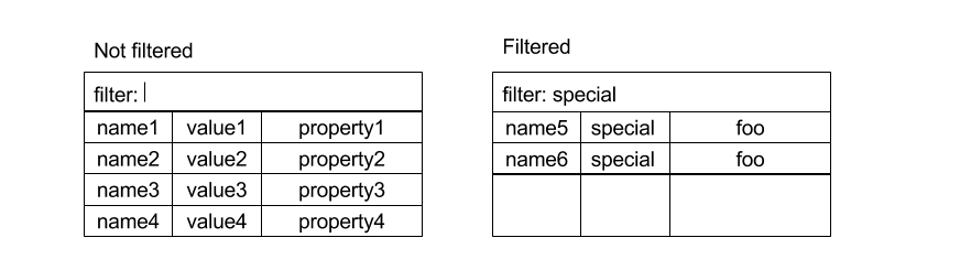
\includegraphics[width=0.75\textwidth]{filtertable}
	\caption{Table component extension example.}
	\label{fig:filtertable}
	\end{figure}

An essential  part of a test for the filter feature is represented in listing
\ref{lst:testbenchTest}. 

 \lstset{style=a1listing}
  \begin{lstlisting} [caption=Example of table test,label={lst:testbenchTest}]
TableElement table = getTableElement();
TextFieldElement filterElement=table.
	$(TextFieldElement.class).id("filter-field").first();
filterElement.setValue("special");

//Comparing filtered values
TableRowElement row=table.getRow(1);
assertEquals(row.getCell(0).getValue(),"special");
  \end{lstlisting}

In addition to having value throughout the development life cycle,
TestBench tests are valuable artifacts to get end-users feedback.
Because TestBench tests are executed in a browser, tests can be used 
for demonstrating framework or application features to an end-user. The key
downside of this approach, that you can not demonstrate the behaviour of the
application till it is written already. In a worst case scenario, a developer
may spend time on implementing features that do not fit user requirements and
have to make tremendous changes after demonstrating the application to the end
user. Using Behaviour Driven Development (BDD) \ref{bddArticle2} technique helps
to improve this situation.

Behaviour Driven Development is a software development process which combines
TDD and domain driven design. The key to success of BDD is the executable
acceptance tests that describe the expected behavior of a feature and its
acceptance criteria in the form of scenarios using simple and
business people readable syntax\cite{bddArticle}. BDD uses a business readable
language to describe software's behavior while hiding its implementation
details.

During a BDD process a business user works with a business analyst
to identify business requirements. These requirements are expressed as a story
using the following template:

\begin{description}
  \item[Given] an initial context.
  \item[When] an event occurs,
  \item[Then] get some outcomes. 
\end{description}

Business and technology should refer to the same system in the same way, that is
why BDD relies on the use of a very specific and small vocabulary to minimise miscommunication \cite{bddWebSite}.
Because a developer and an end-user are using same language, it is much easier
to negotiate about application requirements and as a result make developing
process faster and more agile.

In the next section we will show how to improve this test by using
BDD framework.

\section{Integrating with Behaviour-Driven Development frameworks}

The main goal of BDD is to get executable specifications of a system.
In other words BDD frameworks allow  to write user-stories in
common language, for example English, and associate them with automated
acceptance tests.

TestBench can be integrated with such BDD frameworks as JBehave
\cite{jBehaveSite} or Cucumber\cite{cucumberSite}.
Tests in JBehave are called scenarios see example of JBehave scenario
\ref{lst:scenario}.

 \lstset{style=console}
  \begin{lstlisting} [caption=JBehave scenario,label={lst:scenario}]
Scenario: filter table contents
Given web-page with table
When typing special to filter field
Then value in row 1 and cell 0 is special
  \end{lstlisting}
User story steps are matched into actual Java tests using annotations. 
The method with an annotation interact with an application and perform the actions needed.
Since TestBench tests are pure Java code and BDD steps can be run as JUnit tests, we can combine these to make
JBehave run TestBench tests.

We start by extending the TestBenchTestCase  and use JBehave's ``\@BeforeScenario''
annotation to open a tested Web page.  @Given @When and @Then annotations are
linked with corresponding steps in the user scenario.
To pass parameters from the user-scenario step to a Java method "\$"- special symbol is used.
JBehave implicitly casts passed value to a parameters type. The complete example
of the test is in appendix A \ref{lst:testbenchTest}.

To link a Java class and a textual story file we need to create a configuration class.
The simplest configuration is a one-to-one mapping between a Java class and a textual story file
see example in appendix A \ref{lst:jbehaveConfig}. 

So we can have both a user-story for our test explaining what should be done and a browser executed
test showing the actual implementation. We believe that user-stories 
greatly ease communication between stakeholders, 
especially if some of them do not have relevant technical background.
So user-stories can be shared between stakeholders to show what is done and what
is planning to be done, if there are questions 
executing these user-stories in a browser will help to reveal more details about it. 
